\section{Planning an NDN network with scalability in mind}
% first discuss how this all comes together; use case --> related work --> mccabe's --> tosca --> poc
This section will discuss the method we used in order to plan an NDN network with scalability in mind. Scalability is defined as capacity to be changed in size or scale. In order to plan an NDN network with this goal in mind we will use a combination of McCabe (section \ref{overview-mccabe}) and TOSCA (section \ref{overview-tosca}). McCabe will function as a method to guide design choices with scalability and performance requirements in mind. While TOSCA will function as an implementation method that provides the means to control the whole life cycle of the network design with scalability and performance in mind as well. Furthermore, a proof of concept will be discussed that we implemented in a limited scope in order to proof the method in practice.

\subsection{Design requirements and analysis (McCabe)}
% define relationships must be more explicit here --> can be used in tosca section then as well as input
In this section we will apply McCabe's approach in order to establish the design requirements and analyze the properties of NDN and how it can be applied to solve the use case of SeaDataCloud. The use case of SeaDataCloud (section \ref{introduction-background}) calls for data request distribution. NDN is designed to make data distribution possible and is gaining popularity in big science. Another requirement is flexible scalability, this will be addressed in the design. The first step is to make an overview of the requirements and known NDN scalability and performance issues.

The following analysis is based on the design requirements and will provide a baseline for the high-level network design. As discussed in the related work (section \ref{introduction-related-work}), several key scalability and performance metrics were highlighted. Several NDN-specific design choices need to be made. These include the consideration that NDN is an overlay, on top of e.g. TCP/IP. Within this context it was concluded that TCP provided the most satisfying performance when compared to UDP. Furthermore, there are several NDN strategies to choose from. The 'leave copy everywhere' cache decision strategy and the 'least recently used' cache replacement strategy were considered to be the overall best performing choices. However, for the forward strategies there was no decisive conclusion on which a selection could be based on. Therefore, we will use the default forwarding strategy; best-route. The performance configurations mentioned can be configured in the \texttt{nfd.conf} file of the NDN-CXX\footnote{\url{https://github.com/named-data/ndn-cxx}} application. NDN-CXX is one of the most mature software implementations of NDN and therefore used in our design. Other performance optimization solutions which were mentioned in the related work require changes in the source-code, which is outside the scope of this research.

\subsection{Architecture (McCabe)}
With the design requirements established we can develop a high-level network design. As mentioned in section \ref{overview-virtualization}, virtualization allows the flexible allocation of cloud resources via VMs and scalability of software application by the use of containers. In order to ease NDN scalability, different data centers can be used to deploy NDN nodes. These nodes can then provide locally cached copies of data objects. And thus providing data distribution which lowers the chance of network congestion for SeaDataCloud.

In figure \ref{fig:high-level-network-design} we illustrate our high-level network design. 

\begin{figure}[H]
\centering
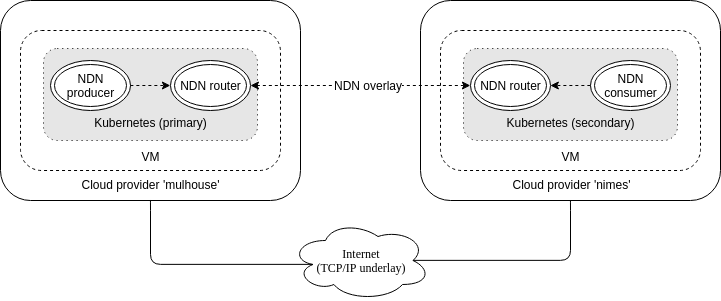
\includegraphics[width=\columnwidth]{Images/high-level-network-design.png}
\caption{High-level network design.}
\label{fig:high-level-network-design}
\end{figure}



% use that as input for mccabe's method of planning a network
% goal: higher throughput, distributed load, flexible scaling
% use performance as input --> i suppose can only be used for deployment strategy (vm's --> docker), or be creative; append own method for this research
% this has as output the network diagram and certain requirements - briefly describe these requirements


% these then have to be merged into a tosca diagram
% describe tosca, applied with input from mccabe
% explain tosca diagram, the features, how it could meet the requirements defined by mccabe


% then describe what will be proven with the proof of concept
% that would be that tosca isn't implemented, but kubernetes its config is used as an abstraction for this
% with kubernetes its config the ndn network can be controlled in an sdn-style way
% describe ndn docker containers (how they can be controlled via kubernetes)
% conclude with the result of easy scaling an ndn network




\subsection{Planning an NDN network}
\label{method-planning}
% Merge McCabe's method and tosca as one method

Merge McCabe + TOSCA, use related work with NDN known performance bottlenecks/improvements as input

\subsection{NDN scalability}
Methodology explained, why use something, with what goal?

An NDN network uses routers, bandwidth and other resources to provide its users with a service. Therefore, the methodology described in McCabe can be used to plan an NDN network as well. However, traditional network designs focus on capacity planning, which is over-engineering the amount of network capacity needed. In NDN, with in-network caching, network traffic is distributed by design. Therefore, McCabe's systems methodology will be used, but slightly adapted to NDN. 